\documentclass[12pt,a4paper]{extarticle}

\usepackage[top=20mm, bottom=20mm, left=30mm, right=20mm]{geometry}
\usepackage[T1]{fontenc}
\usepackage[utf8x]{inputenc}
\usepackage[russian]{babel}
\usepackage{amsmath}
\usepackage{amssymb}
\usepackage{hyperref}
\usepackage{graphicx}
\usepackage{subcaption}


\newcommand{\R}{\mathbb{R}}
\newcommand{\E}{\mathcal{E}}
\newcommand{\W}{\textbf{W}}
\newcommand{\s}{\textbf{s}}
\newcommand{\Loss}{\mathcal{L}}
\newcommand{\encoder}{\operatorname{enc}}
\newcommand{\decoder}{\operatorname{dec}}
\newcommand{\unit}[1]{\textbf{e}_{#1}}

\DeclareMathOperator*{\argmin}{arg\,min}

\title{Анализ проблемы вложения графов и применимости к ней нового метода -- структурной функции потерь}

\begin{document}

    \begin{titlepage}
        \pagenumbering{gobble}
        \clearpage
        \pagestyle{empty}

        \begin{center}
            \textrm{Министерство образования и науки Российской Федерации}
            \\[5mm]
            Федеральное государственное автономное образовательное учреждение\\
            высшего профессионального образования\\
            <<Московский физико-технический институт\\
            {(государственный университет)}>>\\[5mm]
            Факультет радиотехники и кибернетики\\[5mm]
            Кафедра проблем передачи информации и анализа данных\\[50mm]
            \textbf{АНАЛИЗ ПРОБЛЕМЫ ВЛОЖЕНИЯ ГРАФОВ И ПРИМЕНИМОСТИ К НЕЙ НОВОГО МЕТОДА -- СТРУКТУРНОЙ ФУНКЦИИ ПОТЕРЬ}
            \\[8mm]
            \textrm{Выпускная квалификационная работа}
            \\
            (бакалаврская работа)\\[7mm]

            Направление подготовки: 03.03.01 Прикладные математика и физика\\[40mm]
        \end{center}

        \noindent Выполнил:\\
        студент 411а группы \hspace{0.9cm} \underline{\hspace{4cm}} Цепа Станислав Евгеньевич\\[2mm]

        \noindent Научный руководитель:\\
        к.ф.-м.н. \hspace{3.1cm} \underline{\hspace{4cm}} Панов Максим Евгеньевич
        \\[20mm]

        \begin{center}
            Москва 2018
        \end{center}

    \end{titlepage}

    \pagenumbering{arabic}
    \setcounter{page}{2}

    \tableofcontents

    \newpage

    \section{Введение}
    Большинство алгоритмов машинного обучения основано на использовании
    признаков, являющихся числами (а также иногда категориями).
    Однако, далеко не все сущности, которые хотелось бы использовать в качестве признаков,
    можно легко перевести в числовой вид.
    Примерами таких объектов являются слова в тексте или вершины в графе.
    В нашей работе мы рассматривали задачу вложения: как каждой отдельной сущности (в нашем
    случае вершине графа) сопоставить точку вещественного $n$-мерного пространства,
    или, проще говоря, $n$ вещественных чисел, чтобы относительное
    расположение этих точек лучшим образом отображало структуру графа.
    
    Мы предлагаем принципиально новый метод вложения.
    Его основная идея в том, чтобы выделить статистическую характеристику и оптимизировать ее методом стохастического градиентного спуска.
    Преимущества нашего метода -- это простота и возможность переиспользования в других областях машинного обучения, например классификации картинок.
    Мы проверяем качество вложения тремя способами, сравнивая результаты с уже существующими алгоритмами.

    \section{Постановка задачи}
    В данном разделе мы формализуем задачу вложения графов и демонстрируем как можно разделить ее на подзадачи. Наша формализация основана на формализации приведенной в \cite{survey2}.

    Пусть дан невзвешеный граф $G = (V, E)$, $n = |V|$ его матрица смежности $A \in \R^{n \times n},\ A_{ij} \in \{0, 1\}$.
    
    Также вводится матрица схожести $S,\ S_{ij} \in \R_{+}$,  каждый элемент которой оценивает некую "схожесть" двух вершин. Обычно матрицу схожести получают из матрицы смежности таким образом чтобы учитывалось соседство второго и более высших порядков. Стоит заметить, что не во всех алгоритмах возможно использовать небинарную матрицу, например в нашем алгоритме это возоможно только при некоторых усложнениях, поэтому, хоть далее мы и будем для общности везде указывать матрицу $S$, в основном будет подразумеваться $S = A$.
    
    Алгоритм, строящий вложение графа по этим данным, обычно состоит из следующих частей:
    \begin{itemize}
        \item функция кодирования (\textit{encoder}) строит вложение графа
            \[\encoder: V \to \R^{n \times d}.\]
            далее будем обозначать вложение $i$ вершины $\E_i = \encoder(v_i)$
        \item функция декодирования (\textit{decoder}) оценивает схожесть двух элементов вложения,
            в идеальном случае $\decoder(\E_i, \E_j) = S_{ij}$
            \[\decoder: \R^{d} \times \R^{d} \to \R_+\]
        \item функция потерь (\textit{loss}) $\Loss$ оценивает насколько хорошо функции декодирования удалось восстановить исходную матрицу схожести.
    \end{itemize}
    
    Таким образом задача вложения графа сводится к поиску подходящего функционала кодирования и выбора правильной функции потерь, после чего решается задача оптимизации, например при помощи градиентного спуска или аналитически. Далее мы рассмотрим каждую из составляющих алгоритма подробнее.

    \subsection{Функция кодирования}
    Запишем еще раз определение функции кодирования
    \begin{equation}
        \encoder(v_i) = \E\unit{i}.
    \end{equation}
    Здесь $\E$ -- матрица вложения размера $n \times d$, а $\unit{i}$ -- единичный вектор. Можно представить
    \begin{equation} \label{enc_eq_f}
        \encoder(v_i) = f(\s_i),
    \end{equation}
    где $f$ -- произовольная функция $\R^n \to \R^d$, а $\s_i$ -- $i$ столбец матрицы схожести. Этот подход реализуется, например, при использовании нейросетей TODO.
    Если принять, что $f$ линейная функция, то \eqref{enc_eq_f} превратится в
    \begin{equation}
        \encoder(v_i) = \W\s_i + \textbf{b}.
    \end{equation}
    или
    \begin{equation}
        \E = \W S + \textbf{b}.
    \end{equation}
    
    Здесь размер матриц $\W$ и $\textbf{b}$ это $n \times d$. Этой формулой мы и будем пользоваться в нашем алгоритме.
    Стоит заметить что если матрица $S$ имеет ранг хотя бы $d$ то матрица $\E$ может принимать любые значения.

    \subsection{Функция декодирования}
    Функция декодирования обычно имеет простой вид, поскольку она просто представляет из себя вычисление какого либо расстояния между двумя $d$-мерными векторами. Вот примеры такой функции:
    \begin{itemize}
        \item расстояние
            \begin{equation} \label{dec_dist}
            \decoder(\E_i, \E_j) = \lVert \E_i - \E_j \rVert_2 ^ 2
            \end{equation}
        \item скалярное произведение
            \begin{equation} \label{dec_scal}
            \decoder(\E_i, \E_j) = \E_i^T\E_j
            \end{equation}
        \item корреляция, нормированное скалярное произведение
            \begin{equation} \label{corr}
            \decoder(\E_i, \E_j) =  \frac{\E_i^T\E_j}{|\E_i||\E_j|}
            \end{equation}
        \item софтмакс
            \[\decoder(\E_i, \E_j) = \frac{e^{\E_i^T\E_j}}{\sum_{k \in V} e^{\E_i^T\E_k}}\]
    \end{itemize}
    
    \subsection{Функция потерь}
    Существующие функции потерь могут быть условно разделены на два класса: попарная функция потерь и глобальная функция потерь
    
    \subsubsection{Попарная функция потерь}
    Эта функция потерь представляет из себя сумму ошибок по каждому элементу $S$
    
    \begin{equation} \label{pair_loss}
        \Loss = \sum_{i, j \in V} \ell (\decoder(\encoder(v_i), \encoder(v_j)), S_{ij})
    \end{equation}
    
    обычно функция $\ell$ представляет из себя квадратичную ошибку 
    \begin{equation} \label{pair_loss_dist}
    \ell(x, y) = \lVert x - y \rVert_2^2
    \end{equation}
    
    \subsubsection{Глобальная функция потерь}
    В некоторых случаях функция потерь имеет более сложный вид и не может быть разложена в сумму, каждый такой случай можно рассматривать отдельно. К такому виду функции потерь относится и структурная функция потерь -- она пытается вычислять оптимальность вложения основываясь на его статистических характеристиках.

    \section{Обзор алгоритмов}
    Среди уже существующих алгоритмов можно выделить несколько основных групп: методы на основе разложения матриц, методы на основе случайных блужданий, методы на основе нейронных сетей, далее мы рассмотрим эти методы подробнее.
    \subsection{Методы на основе разложения матриц}
    \subsubsection{Laplacian Eigenmaps \cite{laplacianeigenmaps}}
    В алгоритме Laplcian Eigenmaps оптимизируется следующая функция
    \begin{equation} \label{lapl_loss}
        \Loss = \frac{1}{2} \sum_{i, j \in V} \lVert \E_i - \E_j \rVert_2 ^ 2 S_{ij}.
    \end{equation}
    Видно что эта функция является \eqref{pair_loss} с функцией декодирования \eqref{dec_dist} и $\ell(x, y) = xy$.
    
    
    \subsubsection{HOPE \cite{HOPE}}
    
    В алгоритме HOPE вложение получается засчет минимизации
    \[
    \Loss = \lVert S - \E \E^T \rVert.
    \]
    Эта функция минизируется засчет сингулярного разложения и выбора $d$ наибольших сингулярных векторов. Этот алгоритм примечателен тем, что в нем может использоваться любая матрица схожести, в том числе для взвешенного и ориентированного графа.
    Здесь функция декодирования это скалярное произведение \eqref{dec_scal}, а функция $\ell$ -- \eqref{pair_loss_dist}.
    
    \subsection{Методы на основе случайных блужданий}
    Метод случайных блужданий заключается в том что граф переводится в набор признаков описывающих локальное сосество вершин, и далее решается задача из области обработки текстовой информации (\textit{word embedding}). В приведенных ниже примерах применяется широко распространенный алгоритм word2vec.
    
    \subsubsection{Deepwalk \cite{deepwalk}}
    Для данного графа и стартовой точки на каждом шаге мы случайно выбираем соседнюю вершину и перемещаемся в нее, продолжая так определенное количество итераций.
    Запоминая результат, мы получаем последовательность вершин, которая называется случайным блужданием на графе.
    Далее каждая вершина интерпретируется как слово, а одно случайное блуждание как предложение.
    Используя механизм поиска скрытых представлений для слов word2vec, методы получают искомое вложение для вершин графа.
    В данном алгоритме переходы в любую соседнюю вершину равновероятны.
    
    \subsubsection{Node2Vec \cite{node2vec}}
    Данный алгоритм является усовершенствованием алгоритма
    Deepwalk.
    Основное отличие заключается в том, что процесс блуждания регулируется двумя параметрами $p$ и $q$, контролирующими вероятность возвращения в вершину и, соответственно, удаления от вершины.
    Путем настройки этих параметров удается подобрать блуждания, лучше соответствующие структуре конкретного графа.
    
    \subsection{Методы на основе нейронных сетей}
    Стоит заметить что задача вложения является задачей обучения без учителя, поэтому методы на основе нейронных сетей необходимо сперва адаптировать для использования в задачах без учителя.
    Одним из вариантов такой адаптации является использование автоэнкодера -- сети в которой выходной слой равен по размеру входному, а посередине слой размером с искомое вложение.
    Таким образом, если алгоритму оптимизации удастся максимально приблизить выходной слой к входному то данные из срединного слоя можно будет считать вложением.
    Одним из широко распространенных методов на основе нейрнонных сетей является SDNE \cite{sdne}.
    
    \subsection{Методы получения матрицы схожести}
    Также стоит обсудить различные подходы к получению матрицы схожести из матрицы смежности.
    Чаще всего это преобразование преследует цель добавить в матрицу смежности информацию о соседстве второго и более высоких порядков, чтобы алгоритмы вложения работали более эффективно.
    \subsubsection{Метод общих соседей}
    Это самый простой метод, в котором $S_{ij}$ равняется количеству общих соседей у вершин $i$ и $j$:
    \[S = A^2.\]
    \subsubsection{Adamic-adar}
    Этот метод можно назвать взвешенным методом общих соседей, здесь
    \[S = A D A,\]
    где D это диагональная матрица,
    \[D_{ii} = \frac{1}{\sum_{j=1}^n A_{ij}}.\]
    Обычно этот метод более удобен благодаря нормировке.
    
    \section{Структурная функция потерь}
    
    Основная идея нашего исследования заключалась в том, чтобы найти такую статистическую характеристику вложения, оптимизируя которую (при помощи градиентного спуска), мы бы получили вложение, сравнимое по качеству с существующими признаными алгоритмами.
    Ниже приведена финальная реализация нашего алгоритма.
    
    \subsection{Описание алгоритма}
    
    Для каждой пары вершин $u$, $v$ определим соединены ли они ребром (положительная пара) или нет (отрицательная пара). Определим 
    \begin{flalign*}
        a_{uv} =  \begin{cases}
        1,  & \text{если } (u, v) \in E,  \\
        0,  & \text{если } (u, v) \notin E. \\
        \end{cases}
    \end{flalign*}
    	
    Легко заметить что $a_{uv}$ есть не что иное как элементы матрицы смежности (в случае невзвешенного графа). 
    То есть положительные пары для графа $G = (V, E)$ это все ребра $(u, v) \in E$, отрицательные -- ребра $(u, v) \notin E$ соответственно.
    
    Далее случайным образом инициализируем матрицы $\W$ и $\textbf{b}$, это будут матрицы параметров для нашего градиентного спуска и вычислим
    \[\E = \W S + \textbf{b}.\]
    
    Здесь в уравнение входит матрица схожести $S$, но пока считаем, что $S = A$.
    
    После произведем попарное вычисление расстояния между для каждого элемента вложения
    
    \[l_{uv} = \decoder(\E_u, \E_v).\]
    
    В качестве функции $\decoder$ решено было выбрать корреляцию \eqref{corr}. В этом случае $l_{uv} \in [-1, 1]$, что будет удобно для дальнейшего использования.
    
    И наконец, разобьем подсчитанные $l_{uv}$ на два множества в соответсвии с тем к какой паре, положительной или отрицательной, относится $(u, v)$.
    
    \begin{flalign*}
    	L^+ &= \{ l_{uv} =  \decoder(\E_u, \E_v) \mid a_{uv} = 1 \}, \\
    	L^- &= \{ l_{uv} =  \decoder(\E_u, \E_v) \mid a_{uv} = 0 \}.
    \end{flalign*}
    
    В итоге мы получили два множества значений попарных корреляций $L^+$ и $L^-$.
    
    Наш подход основан на эвристике, что вложение будет хорошим если значения внутри $L^+$ будут максимально близки к 1, а внутри $L^-$ максимально близки к 0.
    Мы выбираем не -1 (минимальное значение корреляции), а 0 потому что стремимся получить линейно независимые вложения для отрицательных пар.
    
    Чтобы формализовать эту эвристику мы прибегаем к следующему подходу: посторим два вероятностных распределения при помощи методов непараметрической оценки полтности: $P^+$, $P^-$. Также построим две гистограммы соответствующие этим распределениям с количеством бинов $bin$: $H^+$ и $H^-$.
    
    Определим нашу функцию потерь как
    \[\Loss = D(H^-, H^+),\]
    где $D$ -- функция вычисления расстояния между распределениями (\textit{divergence}). Одна из интересных особенностей нашего алгоритма (и отличие от \cite{hist_loss}) в том, что в качестве $D$ мы используем усовершенствованное расстояние Вассерштайна \cite{emd} для одномерного случая.
    
    Одномерное расстояние Вассерштнайна (также называется \textit{earth mover distance}, \textit{EMD}) определяется как
    \begin{equation} \label{EMD}
        EMD(H_1, H_2) = \sum_{i=1}^{bin} |\varphi_i|,\ \text{где } \varphi_i = \sum_{j=1}^i \left(\frac{H_{1j}}{\lVert H_1 \rVert_1} - \frac{H_{2j}}{\lVert H_2 \rVert_1} \right).
    \end{equation}
    
    Однако, оно обладает тем недостатком, что $EMD(H_1, H_2) = EMD(H_2, H_1)$.
    В нашем случае мы знаем что ситуация, когда $H^+$ левее $H^-$ не симметрична, а наоборот, антисимметрична. Оказывается, если отказаться в \eqref{EMD} от модуля, то новая метрика как раз будет удовлетворять этому условию.
    \begin{equation} \label{EMD_asym}
        EMD_{asym}(H_1, H_2) = \sum_{i=1}^{bin} \varphi_i,\ \text{где } \varphi_i = \sum_{j=1}^i \left(\frac{H_{1j}}{\lVert H_1 \rVert_1} - \frac{H_{2j}}{\lVert H_2 \rVert_1} \right),
    \end{equation}
    \[EMD_{asym}(H_1, H_2) = - EMD_{asym}(H_2, H_1).\]
    
    Расстояние Вассерштайна было выбрано потому, что его оптимизация не только уменьшает пересечение между двумя распределениями, но и стремится максимально <<раздвинуть>> их, поэтому при применении \eqref{EMD_asym} $H^-$ слишком сильно <<уезжала>> влево к значению -1.
    Однако в оптимальном вложении значения из $H^-$ должны быть как можно ближе к 0 для того чтобы быть линейно независимыми.
    Чтобы обойти эту проблему мы решили отбрасывать из $P^-$ все значения с $x < 0$.
    Таким образом к 0 смещались только те значения которые были больше 0, а остальные оставались зафиксированны.
    
    \begin{flalign*}
        P^-_{cut}(x) =  \begin{cases}
        P^-(x)&, \text{если } x \in [0, 1]  \\
        0     &, \text{если } x \in [-1, 0). \\
        \end{cases}
    \end{flalign*}
    
    Итак, 
    \begin{equation}
        \Loss = D(H^-_{cut}, H^+) = EMD_{asym}(H^-_{cut}, H^+).
    \end{equation}
    
    Запишем итоговую задачу оптимизации
    \begin{equation} \label{optimization_task}
    \W_{opt}, \mathbf{b}_{opt} = \argmin_{\W, \mathbf{b}} \Loss,
    \end{equation}
    \[\E_{opt} = \W_{opt} S + \mathbf{b}_{opt}.\]
    
    
    \section{Эксперименты}
    В данном разделе приведено экспериментальное исследование нашего алгоритма. Оптимизация \eqref{optimization_task} производилась при помощи библиотеки Tensorflow.
    Код всех экспериментов доступен на \url{https://github.com/premolab/GraphEmbeddings}.
    
    \subsection{Данные для экспериментов}
    
    В качестве данных для экспериментов были использованы графы размером от 100 до 10000 вершин.
    Все графы являются либо модельными, либо реальными графами, часто используемыми для исследования алгоритмов. Данные о графах приведены в таблице \ref{table_graphs}.
    Граф SBM (\textit{Stochastic Block Model}) является модельным графом с 900 вершинами. Сперва вершины разбиваются на три группы, а затем ребра добавляются случайным образом: между вершинами одной группы -- с вероятностью $p_{in}$, между вершинами разных групп -- с вероятностью $p_{out}$. Значения $p_{in}$ и $p_{out}$ в наших экспериментах: $p_{in} \in \{0.08, 0.1\}$, $p_{out} \in \{0.01, 0.03\}$.
    
    \begin{table}
    \begin{center}
    \begin{tabular}{ccc}
    	Название & Количество вершин & Описание\\
        \noalign{\smallskip}
        \hline
        \noalign{\smallskip}
        American college football & 115 & неориентированый, реальный \\
        Books about US politics & 105 & неориентированый, реальный \\
        BlogCatalog & 10312 & неориентированый, реальный \\
        Facebook & 4039 & неориентированый, реальный \\
        Stochastic Block Model & 900 & неориентированый, модельный
    \end{tabular}
    \end{center}
    \caption{Список графов} \label{table_graphs}
    \end{table}
    
    \subsection{Описание экспериментов}
    
    \subsubsection{Задача классификации}
    
    Эта задача формулируется таким образом: для какой-то части вершин $V$ задана целевая переменная, например класс или бинарный вектор принадлежности к нескольким классам. Необходимо предсказать значение этой целевой переменной для остальных вершин.
    Подход к решению этой задачи, который мы рассматриваем здесь, это 
    \begin{enumerate}
        \item построить вложение $\E = \E(V, E)$ \label{itm:build_E};
        \item решить задачу обучения с учителем на числовых признаках $\E$.
    \end{enumerate}
    
    Стоит отметить, что пункт \ref{itm:build_E} в данном алгоритме все также относится к задачам обучения без учителя, то есть целевая переменная в нем никак не используется.
    
    \subsubsection{Задача кластеризации}
    
    В этой задаче заранее известно разбиение вершин на кластеры (обычно непересекающиеся). Алгоритм почти такой же как и при классификации.
    
    \begin{enumerate}
        \item Построить вложение $\E = \E(V, E)$;
        \item решить задачу кластеризации на числовых признаках $\E$.
    \end{enumerate}
    
    Отличие заключается в том, что все пункты алгоритма относятся к обучению без учителя, а метки кластеров используются лишь при подсчете метрики качества.
    
    \subsubsection{Задача предсказания ребер}
    
    Задача предсказания ребер (\textit{link prediction}) является более универсальным способом оценить качество вложения, поскольку не требует дополнительной целевой переменной. В ней вложение подсчитывается только на части ребер графа, а затем проверяется насколько хорошо по этому вложению можно предсказать пропущенные ребра.
    
    \begin{enumerate}
        \item Разбить случайным образом множество ребер $E$ на две части $E_{train}$ и $E_{test}$;\footnote{Чаще всего накладывается дополнительное требование чтобы $G_{train} = (V, E_{train})$ был связным графом.}\footnote{В нашем случае был выбран такой коэффециент разибения, что $|E_{train}| = |E_{test}| = \frac{|E|}{2}$}
        \item построить вложение $\E = \E(V, E_{train})$;
        \item Выбрать примеры ребер из множеств $E_{train}$ и $E_{test}$ а также отрицательные примеры такие что $(u, v) \notin E$; \label{itm:choose_edges}
        \item определить переменные
            \begin{flalign*}
                y(u, v) =  \begin{cases}
                1, & \text{если } (u, v) \in V,  \\
                0, & \text{если } (u, v) \notin V;  \\
                \end{cases}
            \end{flalign*}
            \[X(u, v) = (\E_u, \E_v),\]
        где $(\cdot\,, \cdot)$ означает конкатенацию;
        \item решить задачу обучения с учителем для данных $X$ и целевой переменной $y$, подсчитанных на примерах из пункта \ref{itm:choose_edges}.
    \end{enumerate}
    
    \subsection{Результаты экспериментов}

    Мы проводили сравнение работы нашего алгоритма с алгоритмами двух других семейств: алгоритмов на случайных блужданиях и алгоритмов с использованием матричной факторизации. Были выбраны алгоритмы показывающие лучшие результаты внутри своих групп: deepwalk и HOPE соответственно.

    \subsubsection{Задача классификации}

    Для данной задачи мы проверяли работу алгоритма на двух графах: BlogCatalog и SBM. Результаты представлены на рисунке \ref{fig:clas}. Результаты классификации нашего алгортитма на BlogCatalog (рис. \ref{fig:clas_blog}) оказались значительно ниже, чем у алгоритма deepwalk. Впрочем, как показывают обзорные статьи \cite{survey}\cite{survey2}, все алгоритмы не относящиеся к семейству алгоритмов на случайных блужданиях дают такие же плохие результаты. На графе SBM наш алгоритм дал результаты сравнимые по качеству с остальными алгоритмами.
    
    \begin{figure}
    \begin{subfigure}{.5\linewidth}
    \centering
    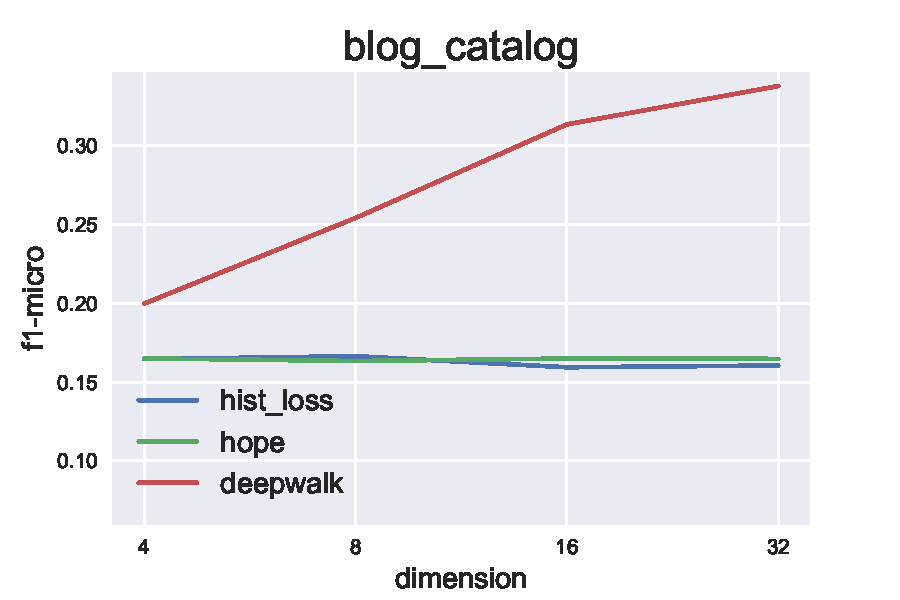
\includegraphics[width=\linewidth]{src/images/Node_classification_blog_catalog.pdf}
    \caption{BlogCatalog}
    \label{fig:clas_blog}
    \end{subfigure}
    \begin{subfigure}{.5\linewidth}
    \centering
    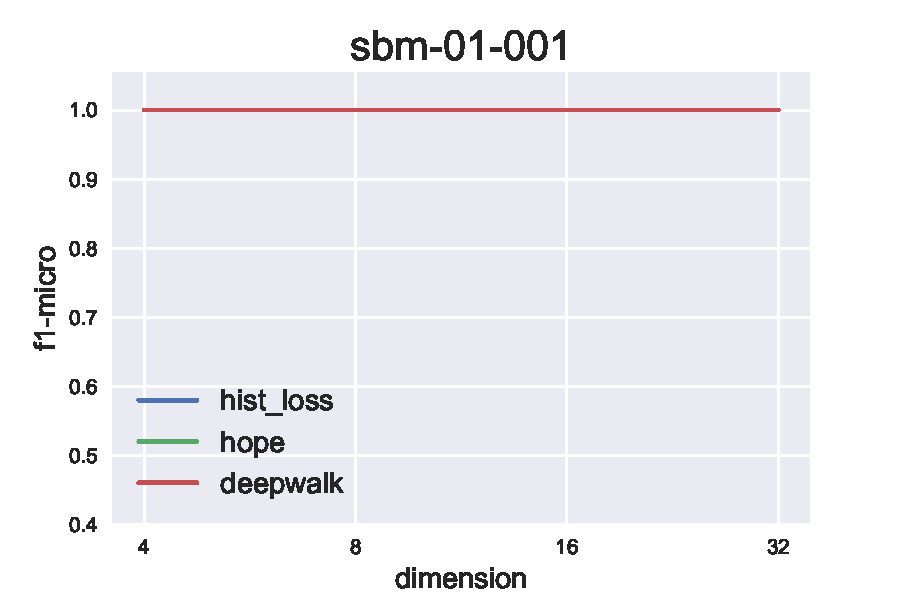
\includegraphics[width=\linewidth]{src/images/Node_classification_sbm-01-001.pdf}
    \caption{SBM $p_{in}=0.1$, $p_{out}=0.01$}
    \label{fig:clas_sbm1}
    \end{subfigure}
    \\[1ex]
    \begin{subfigure}{.5\linewidth}
    \centering
    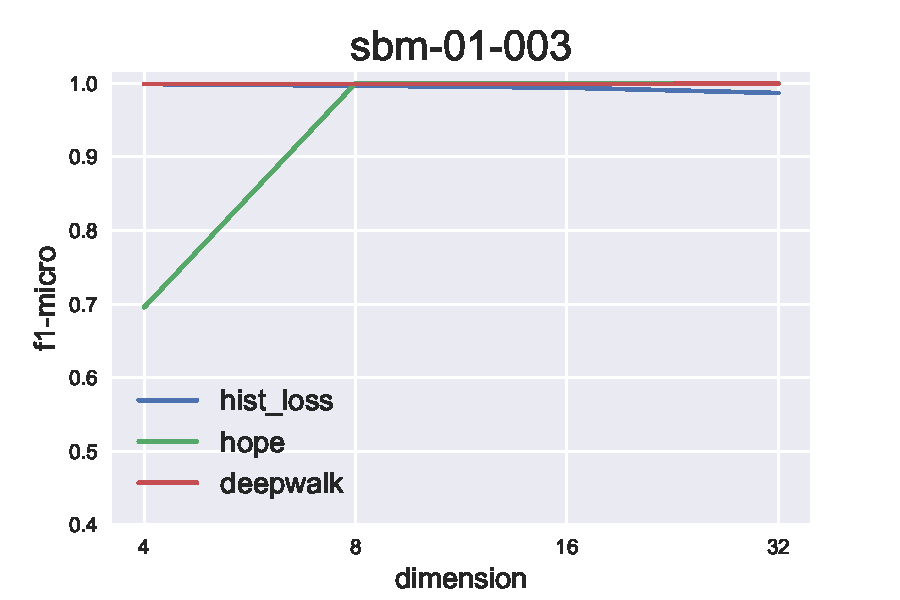
\includegraphics[width=\linewidth]{src/images/Node_classification_sbm-01-003.pdf}
    \caption{SBM $p_{in}=0.1$, $p_{out}=0.03$}
    \label{fig:clas_sbm2}
    \end{subfigure}
    \begin{subfigure}{.5\linewidth}
    \centering
    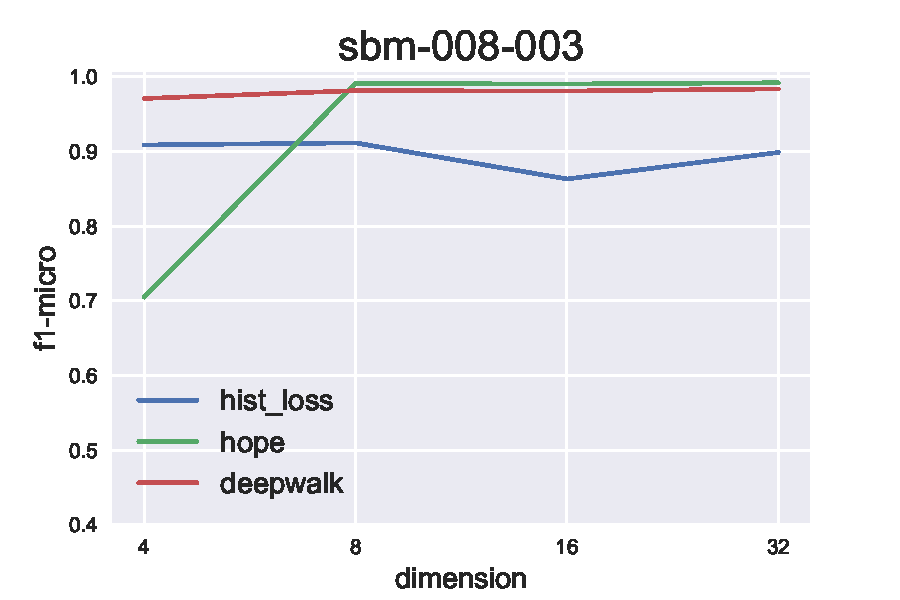
\includegraphics[width=\linewidth]{src/images/Node_classification_sbm-008-003.pdf}
    \caption{SBM $p_{in}=0.08$, $p_{out}=0.03$}
    \label{fig:clas_sbm3}
    \end{subfigure}
    \caption{Результаты классификации}
    \label{fig:clas}
    \end{figure}
    
    \subsubsection{Задача кластеризации}

    Для данной задачи мы проверяли работу алгоритма на графах Football, Political books и SBM, поскольку они имеют метки для кластеризации.
    Результаты представлены на рисунке \ref{fig:clus}.
    Можно заметить, что результаты нашего алгоритма в основном превосходят результаты алгоритма HOPE и приближаются к результатам deepwalk.
    Это ожидаемый результат, поскольку при оптимизации структурной функции потерь все положительные пары ребер приближаются к 1, что в итоге дает очень плотные кластеры.
    
    \begin{figure}
    \begin{subfigure}{.5\linewidth}
    \centering
    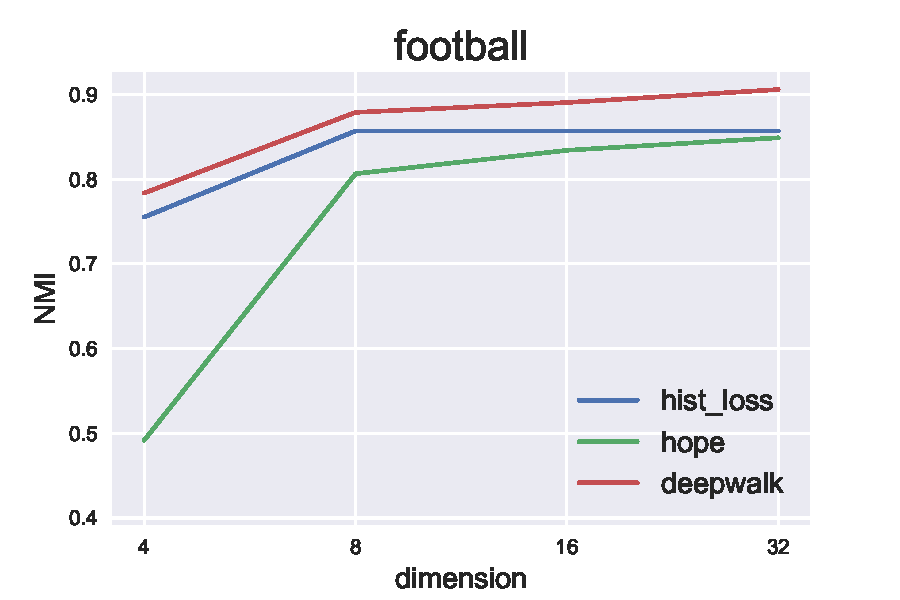
\includegraphics[width=\linewidth]{src/images/Node_clusterization_football.pdf}
    \caption{Football}
    \label{fig:clus_foot}
    \end{subfigure}
    \begin{subfigure}{.5\linewidth}
    \centering
    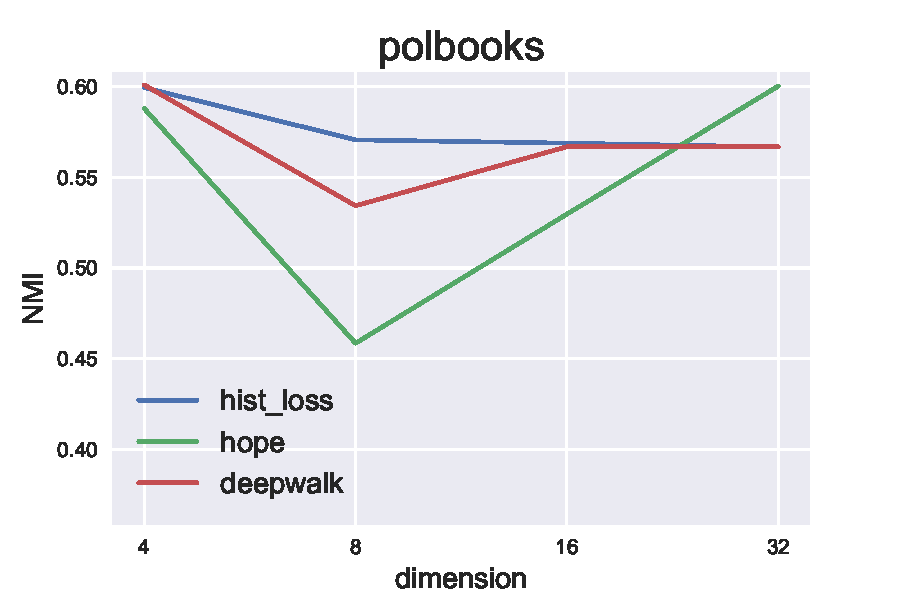
\includegraphics[width=\linewidth]{src/images/Node_clusterization_polbooks.pdf}
    \caption{Political Books}
    \label{fig:clas_pol}
    \end{subfigure}
    \\[1ex]
    \begin{subfigure}{.5\linewidth}
    \centering
    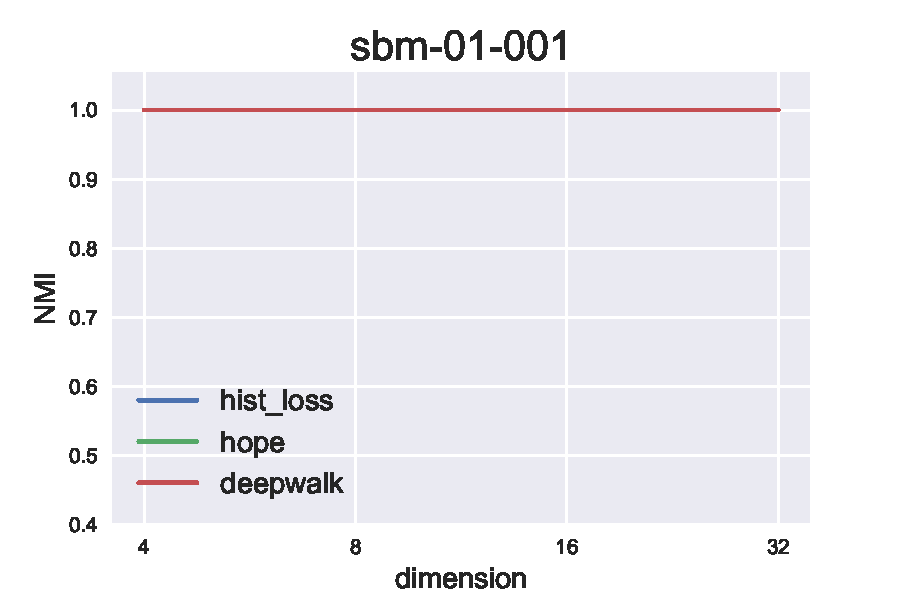
\includegraphics[width=\linewidth]{src/images/Node_clusterization_sbm-01-001.pdf}
    \caption{SBM $p_{in}=0.1$, $p_{out}=0.01$}
    \label{fig:clus_sbm1}
    \end{subfigure}
    \begin{subfigure}{.5\linewidth}
    \centering
    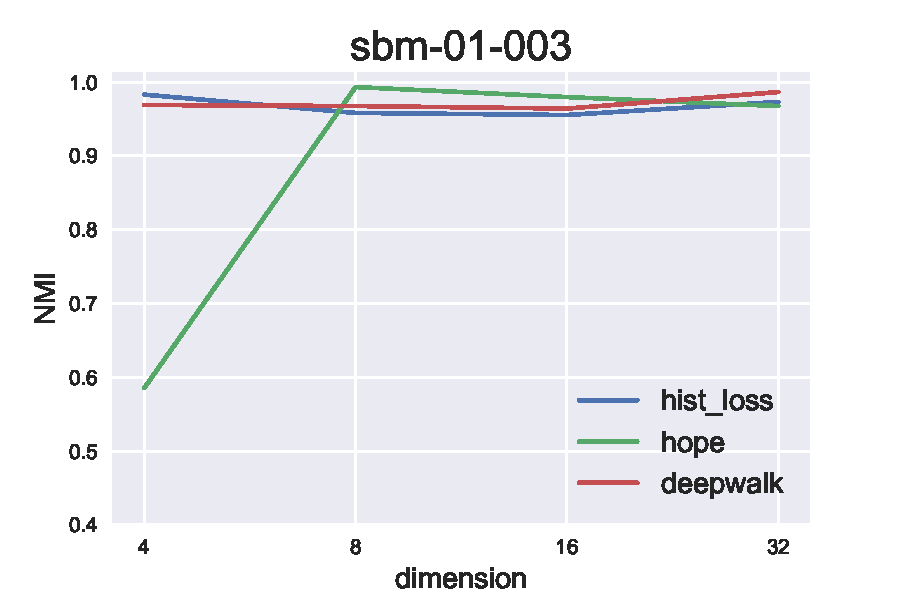
\includegraphics[width=\linewidth]{src/images/Node_clusterization_sbm-01-003.pdf}
    \caption{SBM $p_{in}=0.1$, $p_{out}=0.03$}
    \label{fig:clus_sbm2}
    \end{subfigure}
    \caption{Результаты кластеризации}
    \label{fig:clus}
    \end{figure}
    
    \subsubsection{Задача предсказания ребер}

    Результаты представлены на рисунке \ref{fig:lp}. Видно, что на всех реальных графах наш алгоритм превосходит другие. Это может быть связано со спецификой работы метрики roc-auc, используемой при оценке качества предсказания ребер.
    Метрика roc-auc оценивает разделимость двух классов, в данном случае положительных и отрицательных пар вершин. В то же время структурная функция потерь также зависит от степени разделимости классов, поскольку пытается <<развести>> положительные и отрицательные пары вершин как можно дальше.
    
    \begin{figure}
    \begin{subfigure}{.5\linewidth}
    \centering
    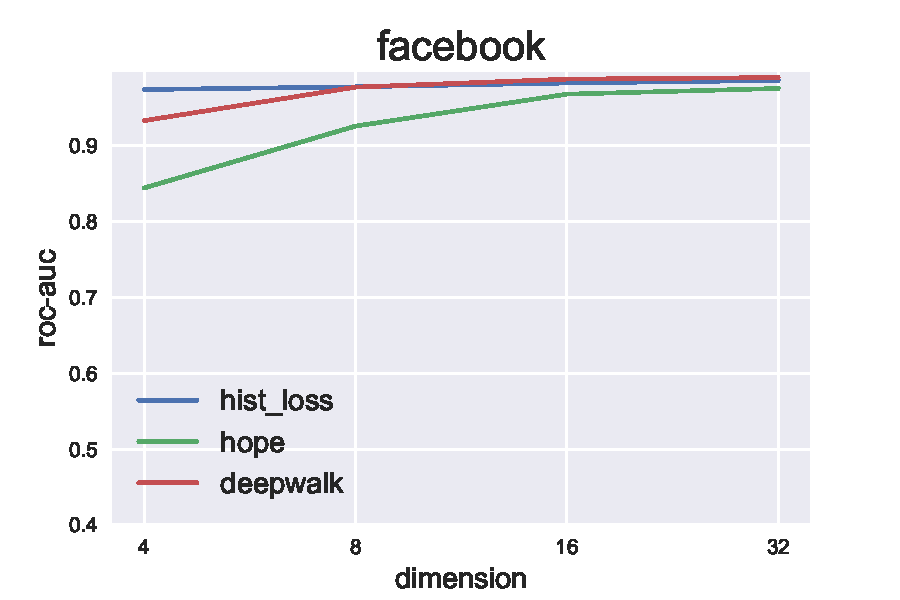
\includegraphics[width=\linewidth]{src/images/Link_prediction_facebook.pdf}
    \caption{Facebook}
    \label{fig:lp_face}
    \end{subfigure}
    \begin{subfigure}{.5\linewidth}
    \centering
    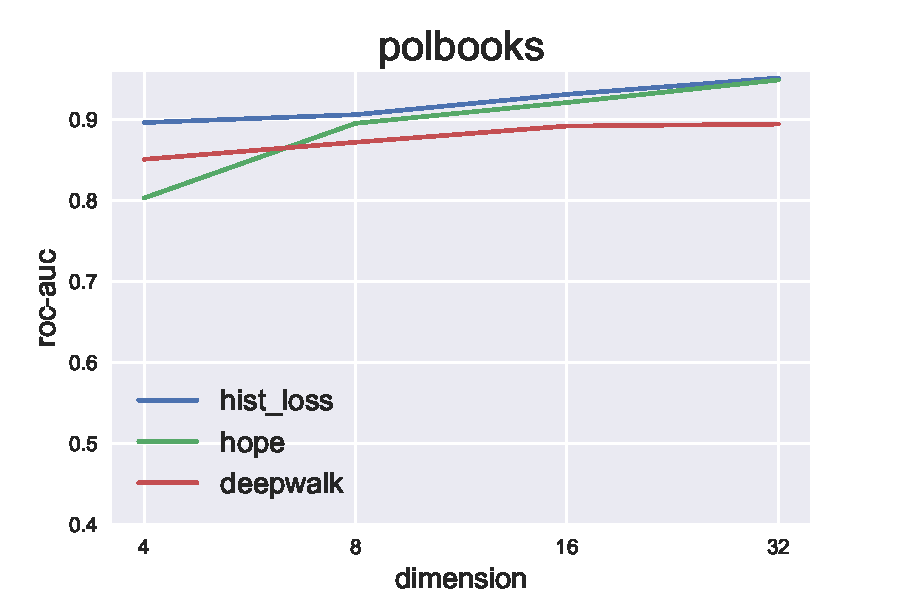
\includegraphics[width=\linewidth]{src/images/Link_prediction_polbooks.pdf}
    \caption{Political Books}
    \label{fig:lp_pol}
    \end{subfigure}
    \\[1ex]
    \begin{subfigure}{.5\linewidth}
    \centering
    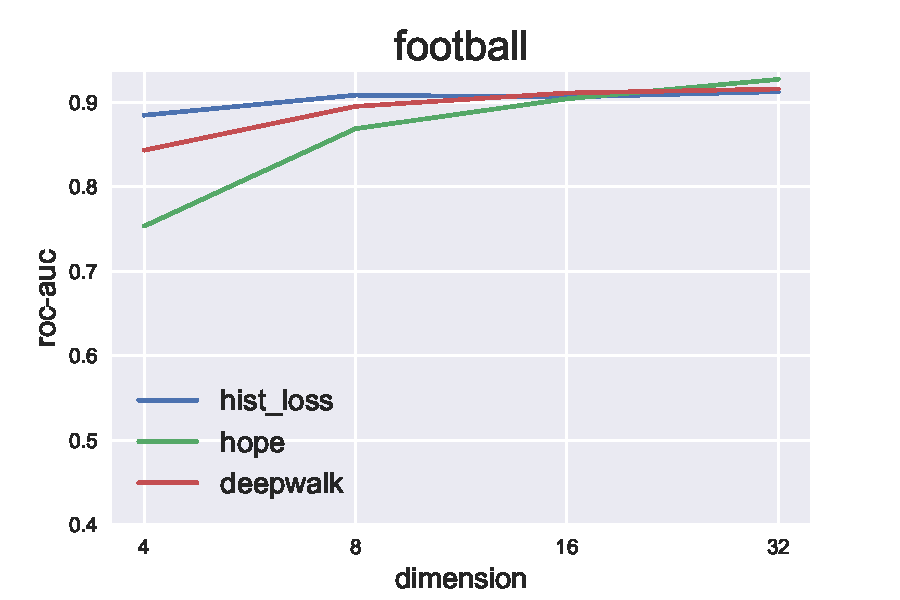
\includegraphics[width=\linewidth]{src/images/Link_prediction_football.pdf}
    \caption{Football}
    \label{fig:lp_foot}
    \end{subfigure}
    \begin{subfigure}{.5\linewidth}
    \centering
    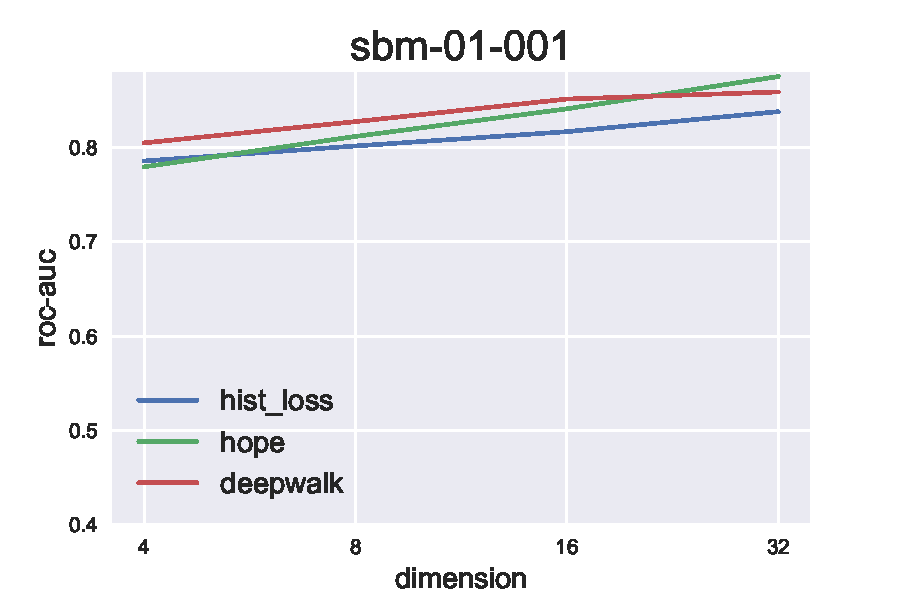
\includegraphics[width=\linewidth]{src/images/Link_prediction_sbm-01-001.pdf}
    \caption{SBM $p_{in}=0.1$, $p_{out}=0.01$}
    \label{fig:lp_sbm1}
    \end{subfigure}
    \\[1ex]
    \begin{subfigure}{.5\linewidth}
    \centering
    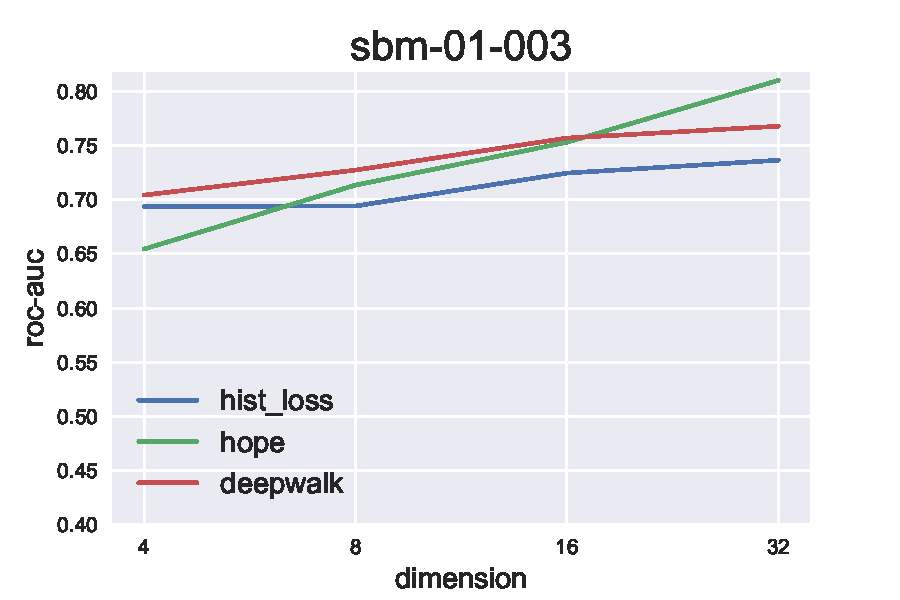
\includegraphics[width=\linewidth]{src/images/Link_prediction_sbm-01-003.pdf}
    \caption{SBM $p_{in}=0.1$, $p_{out}=0.03$}
    \label{fig:lp_sbm2}
    \end{subfigure}
    \caption{Результаты предсказания ребер}
    \label{fig:lp}
    \end{figure}
    
    \section{Выводы}
    
    В данной работе был предложен метод вложения графов, который нельзя отнести ни к одному существующему семейству алгоритмов. Результаты экспериментов показали, что качество работы алгоритма сравнимо с качеством существующих методов, и что структурная функция потерь, при некоторой доработке, может считаться хорошим алгоритмом для вложения. Основные направления для дальнейшей работы: 
    \begin{itemize}
    \item улучшение масштабируемости нашего алгоритма
    
    сейчас время работы алгоритма сильно увеличивается при увеличении размера графа, кроме того построение гистограмм распределений может занимать большое количество оперативной памяти; 
    \item улучшение работы нашего алгоритма с небинарной матрицей схожести
    
    наш алгоритм не рассчитан на небинарные значения $s_{ij}$, поскольку он строится на идее, что все ребра можно разделить на два класса, где $s_{ij}$ принимает значение 0 или 1; были осуществлены попытки бинаризации небинарной $S$, например считать $s_{ij} > threshold \approx 0.1$ положительными примерамм, а остальные отрицательными, но это не дало прироста в качестве работы.
    \end{itemize}
    
    \bibliography{main}
    \bibliographystyle{plain}

\end{document}
